\chapter{Modes of Operation}

\begin{table}[h!]\centering\renewcommand{\arraystretch}{1.05} % Increase row height by 1.5 times
	\caption{Comparison of Modes}
	\begin{tabular*}{\textwidth}{@{\extracolsep{\fill}}c||ccccccc}
		\toprule[1.2pt]
		Mode & Integrity & Authentication & $\EncryptBlk$ & $\DecryptBlk$ & Padding & IV & $\abs{P}\overset{?}{=}\abs{C}$ \\
		\midrule
		$\ECB$ & \yes & \no & \yes & \yes & \yes & \no & $\abs{P}<\abs{C}$ \\
		$\CBC$ & \yes & \no & \yes & \yes & \yes & \yes & $\abs{P}<\abs{C}$ \\
		$\OFB$ & \yes & \no & \yes & \no & \no & \yes & $\abs{P}=\abs{C}$ \\
		$\CFB$ & \yes & \no & \yes & \no & \no & \yes & $\abs{P}=\abs{C}$ \\
		$\CTR$ & \yes & \no & \yes & \no & \no & \yes & $\abs{P}=\abs{C}$ \\
		$\CBCCS$ & \yes & \no & \yes & \yes & \no & \yes & $\abs{P}=\abs{C}$ \\
		\bottomrule[1.2pt]
	\end{tabular*}
\end{table}

\section{Padding}
Block ciphers require input lengths to be a multiple of the block size. Padding is used to extend the last block of plaintext to the required length. Without proper padding, the encryption process may be insecure or infeasible.\\
\\
There are several padding schemes used in practice, such as:
\begin{table}[ht]
	\centering\renewcommand{\arraystretch}{1.05}
	\caption{Padding Standards in Block Ciphers}
	\begin{tabular*}{\textwidth}{>{\bfseries}l||l}
		\toprule
		\textbf{Standard Name} & \textbf{Padding Method} \\
		\midrule
		\multirow{2}{*}{$\mathcolorbox{yellow}{\textbf{PKCS\#7}}$} & Pad with bytes all the same value as the number of padding bytes \\
		& \texttt{\dots dd | dd dd dd dd dd dd dd dd dd dd dd dd \textcolor{red}{04} \textcolor{red}{04} \textcolor{red}{04} \textcolor{red}{04}} | \\
		\hline
		\multirow{2}{*}{ANSI X9.23} & Pad with zeros, last byte is the number of padding bytes \\
		& \texttt{\dots dd | dd dd dd dd dd dd dd dd dd dd dd \textcolor{red}{00} \textcolor{red}{00} \textcolor{red}{00} \textcolor{red}{00} \textcolor{red}{05}} | \\
		\hline
		\multirow{2}{*}{ISO/IEC 7816-4} & First byte is '80' (hex), followed by zeros \\
		& \texttt{\dots dd | dd dd dd dd dd dd dd dd dd dd \textcolor{red}{80} \textcolor{red}{00} \textcolor{red}{00} \textcolor{red}{00} \textcolor{red}{00} \textcolor{red}{00}} | \\
		\hline
		\multirow{2}{*}{ISO 10126} & Pad with random bytes, last byte is the number of padding bytes \\
		& \texttt{\dots dd | dd dd dd dd dd dd dd dd dd dd \textcolor{red}{2e} \textcolor{red}{49} \textcolor{red}{1b} \textcolor{red}{c1} \textcolor{red}{aa} \textcolor{red}{06}} | \\
		\bottomrule
	\end{tabular*}
	\label{tab:padding_standards}
\end{table}

\newpage
\subsection{PKCS\#7}

\begin{lstlisting}[style=C]
void PKCS7_PAD(u32* block, size_t block_len, size_t input_len) {
	if (block_len < input_len) {
		fprintf(stderr,
			"Block length must be greater than input length.\n");
		return;
	}
	
	u8 padding_value = block_len - input_len;
	for (size_t i = input_len; i < block_len; ++i) {
		block[i] = padding_value;
	}
}
\end{lstlisting}

\newpage
\section{$\ECB$ (Electronic CodeBook)}
\begin{algorithm}[H]
	\caption{Electronic CodeBook}
	\begin{multicols}{2}
		\KwIn{$K$ and $P=P_1\parallel\cdots\parallel P_N$ ($P_i\in\binaryfield^{n}$)}
		\KwOut{$C=C_1\parallel\cdots\parallel C_N$ ($C_i\in\binaryfield^n$)}
		\BlankLine
		\For{$i\gets 1$ \KwTo $N$}{
			$C_i\gets\EncryptBlk(K, P_i)$\;
		}
		\Return $C=C_1\parallel\cdots\parallel C_N$\;
		\columnbreak % Move to the next column
		\setcounter{AlgoLine}{0}  % Reset line numbering
		\KwIn{$K$ and $C=C_1\parallel\cdots\parallel C_N$ ($C_i\in\binaryfield^n$)}
		\KwOut{$P=P_1\parallel\cdots\parallel P_N$ ($P_i\in\binaryfield^{n}$)}
		\BlankLine
		\For{$i\gets 1$ \KwTo $N$}{
			$P_i\gets\DecryptBlk(K, C_i)$\;
		}
		\Return $C=C_1\parallel\cdots\parallel C_N$\;
	\end{multicols}
	\BlankLine
\end{algorithm}

\newpage
\section{$\CBC$ (Cipher Block Chaining)}

\begin{algorithm}[H]
	\caption{Cipher Block Chaining}
	\begin{multicols}{2}
		\KwIn{$K$ and $P=P_1\parallel\cdots\parallel P_N$ ($P_i\in\binaryfield^{128}$)}
		\KwOut{$C=C_1\parallel\cdots\parallel C_N$ ($C_i\in\binaryfield^{128}$)}
		\BlankLine
		$C_0\gets IV$\;
		\For{$i\gets 1$ \KwTo $N$}{
			$C_i\gets\EncryptBlk(K, P_i\oplus C_{i-1})$\;
		}
		\Return $C=C_1\parallel\cdots\parallel C_N$\;
		\columnbreak % Move to the next column
		\setcounter{AlgoLine}{0}  % Reset line numbering
		\KwIn{$K$ and $C=C_1\parallel\cdots\parallel C_N$}
		\KwOut{$P=P_1\parallel\cdots\parallel P_N$}
		\BlankLine
		$C_0\gets IV$\;
		\For{$i\gets 1$ \KwTo $N$}{
			$P_i\gets C_{i-1}\oplus\DecryptBlk(K, C_i)$\;
		}
		\Return $P=P_1\parallel\cdots\parallel P_N$\;
	\end{multicols}
	\BlankLine
\end{algorithm}

\begin{center}
\begin{minipage}{.48\textwidth}\centering
\tikzset{every picture/.style={line width=0.75pt}} %set default line width to 0.75pt        
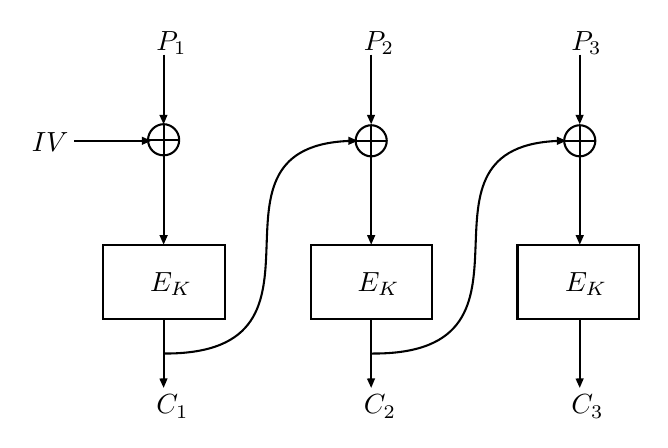
\begin{tikzpicture}[x=0.75pt,y=0.75pt,yscale=-0.5,xscale=0.5]
	% Draw circles and their corresponding lines
	\draw   (136,160) .. controls (136,152) and (143,145) .. (151,145) .. controls (159,145) and (166,152) .. (166,160) .. controls (166,169) and (159,175) .. (151,175) .. controls (143,175) and (136,169) .. (136,160) -- cycle ; 
	\draw   (136,160) -- (166,160) ; 
	\draw   (151,145) -- (151,175) ;
	
	\draw   (336,161) .. controls (336,153) and (343,146) .. (351,146) .. controls (359,146) and (366,153) .. (366,161) .. controls (366,169) and (359,176) .. (351,176) .. controls (343,176) and (336,169) .. (336,161) -- cycle ; 
	\draw   (336,161) -- (366,161) ; 
	\draw   (351,146) -- (351,176) ;
	
	\draw   (537,161) .. controls (537,153) and (544,146) .. (552,146) .. controls (560,146) and (567,153) .. (567,161) .. controls (567,169) and (560,176) .. (552,176) .. controls (544,176) and (537,169) .. (537,161) -- cycle ; 
	\draw   (537,161) -- (567,161) ; 
	\draw   (552,146) -- (552,176) ;
	
	% Draw rectangles
	\draw   (93,261) -- (210,261) -- (210,333) -- (93,333) -- cycle ;
	\draw   (293,261) -- (410,261) -- (410,333) -- (293,333) -- cycle ;
	\draw   (492,261) -- (609,261) -- (609,333) -- (492,333) -- cycle ;
	
	% Draw straight lines
	\draw    (151,78) -- (151,142) ;
	\draw [shift={(151,145)}, rotate = 269] [fill={rgb, 255:red, 0; green, 0; blue, 0 }  ][line width=0.08]  [draw opacity=0] (9,-4) -- (0,0) -- (9,4) -- cycle    ;
	\draw    (351,78) -- (351,142) ;
	\draw [shift={(351,145)}, rotate = 269] [fill={rgb, 255:red, 0; green, 0; blue, 0 }  ][line width=0.08]  [draw opacity=0] (9,-4) -- (0,0) -- (9,4) -- cycle    ;
	\draw    (552,78) -- (552,142) ;
	\draw [shift={(552,145)}, rotate = 269] [fill={rgb, 255:red, 0; green, 0; blue, 0 }  ][line width=0.08]  [draw opacity=0] (9,-4) -- (0,0) -- (9,4) -- cycle    ;
	
	\draw    (65,161) -- (136,161) ;
	\draw [shift={(139,161)}, rotate = 180] [fill={rgb, 255:red, 0; green, 0; blue, 0 }  ][line width=0.08]  [draw opacity=0] (9,-4) -- (0,0) -- (9,4) -- cycle    ;
	\draw    (151,176) -- (151,258) ;
	\draw [shift={(151,261)}, rotate = 270] [fill={rgb, 255:red, 0; green, 0; blue, 0 }  ][line width=0.08]  [draw opacity=0] (9,-4) -- (0,0) -- (9,4) -- cycle    ;
	\draw    (351,176) -- (351,258) ;
	\draw [shift={(351,261)}, rotate = 270] [fill={rgb, 255:red, 0; green, 0; blue, 0 }  ][line width=0.08]  [draw opacity=0] (9,-4) -- (0,0) -- (9,4) -- cycle    ;
	\draw    (552,176) -- (552,258) ;
	\draw [shift={(552,261)}, rotate = 270] [fill={rgb, 255:red, 0; green, 0; blue, 0 }  ][line width=0.08]  [draw opacity=0] (9,-4) -- (0,0) -- (9,4) -- cycle    ;
	
	\draw    (151,333) -- (151,396) ;
	\draw [shift={(151,399)}, rotate = 269] [fill={rgb, 255:red, 0; green, 0; blue, 0 }  ][line width=0.08]  [draw opacity=0] (9,-4) -- (0,0) -- (9,4) -- cycle    ;
	\draw    (351,333) -- (351,396) ;
	\draw [shift={(351,399)}, rotate = 269] [fill={rgb, 255:red, 0; green, 0; blue, 0 }  ][line width=0.08]  [draw opacity=0] (9,-4) -- (0,0) -- (9,4) -- cycle    ;
	\draw    (552,333) -- (552,396) ;
	\draw [shift={(552,399)}, rotate = 269] [fill={rgb, 255:red, 0; green, 0; blue, 0 }  ][line width=0.08]  [draw opacity=0] (9,-4) -- (0,0) -- (9,4) -- cycle    ;
	
	% Draw curved lines
	\draw    (151,366) .. controls (337,367) and (168,163) .. (335,161) ;
	\draw [shift={(338,161)}, rotate = 180] [fill={rgb, 255:red, 0; green, 0; blue, 0 }  ][line width=0.08]  [draw opacity=0] (9,-4) -- (0,0) -- (9,4) -- cycle    ;
	\draw    (352,366) .. controls (538,367) and (370,163) .. (536,161) ;
	\draw [shift={(539,161)}, rotate = 180] [fill={rgb, 255:red, 0; green, 0; blue, 0 }  ][line width=0.08]  [draw opacity=0] (9,-4) -- (0,0) -- (9,4) -- cycle    ;
	
	% Add text nodes
	\draw (141,53) node [anchor=north west][inner sep=0.75pt]    {$P_{1}$};
	\draw (341,53) node [anchor=north west][inner sep=0.75pt]    {$P_{2}$};
	\draw (541,53) node [anchor=north west][inner sep=0.75pt]    {$P_{3}$};
	\draw (21,150) node [anchor=north west][inner sep=0.75pt]    {$IV$};
	\draw (135,285) node [anchor=north west][inner sep=0.75pt]    {$E_{K}$};
	\draw (335,285) node [anchor=north west][inner sep=0.75pt]    {$E_{K}$};
	\draw (535,285) node [anchor=north west][inner sep=0.75pt]    {$E_{K}$};
	\draw (141,403) node [anchor=north west][inner sep=0.75pt]    {$C_{1}$};
	\draw (341,403) node [anchor=north west][inner sep=0.75pt]    {$C_{2}$};
	\draw (541,403) node [anchor=north west][inner sep=0.75pt]    {$C_{3}$};
\end{tikzpicture}
\end{minipage}
\begin{minipage}{.48\textwidth}\centering
\tikzset{every picture/.style={line width=0.75pt}} %set default line width to 0.75pt        
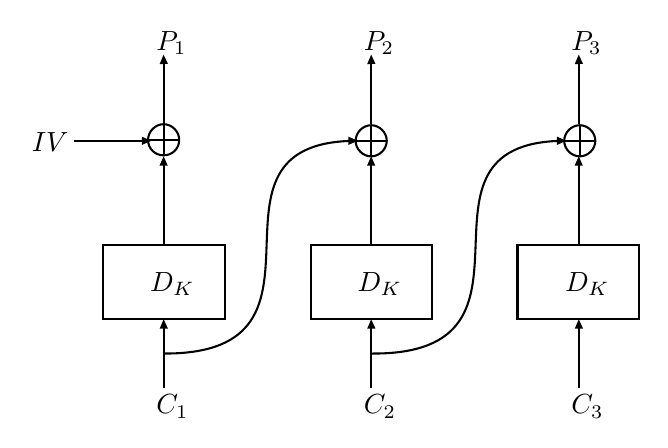
\begin{tikzpicture}[x=0.75pt,y=0.75pt,yscale=-0.5,xscale=0.5]
	% Draw circles and their corresponding lines
	\draw   (136,160) .. controls (136,152) and (143,145) .. (151,145) .. controls (159,145) and (166,152) .. (166,160) .. controls (166,169) and (159,175) .. (151,175) .. controls (143,175) and (136,169) .. (136,160) -- cycle ; 
	\draw   (136,160) -- (166,160) ; 
	\draw   (151,145) -- (151,175) ;
	
	\draw   (336,161) .. controls (336,153) and (343,146) .. (351,146) .. controls (359,146) and (366,153) .. (366,161) .. controls (366,169) and (359,176) .. (351,176) .. controls (343,176) and (336,169) .. (336,161) -- cycle ; 
	\draw   (336,161) -- (366,161) ; 
	\draw   (351,146) -- (351,176) ;
	
	\draw   (537,161) .. controls (537,153) and (544,146) .. (552,146) .. controls (560,146) and (567,153) .. (567,161) .. controls (567,169) and (560,176) .. (552,176) .. controls (544,176) and (537,169) .. (537,161) -- cycle ; 
	\draw   (537,161) -- (567,161) ; 
	\draw   (552,146) -- (552,176) ;
	
	% Draw rectangles
	\draw   (93,261) -- (210,261) -- (210,333) -- (93,333) -- cycle ;
	\draw   (293,261) -- (410,261) -- (410,333) -- (293,333) -- cycle ;
	\draw   (492,261) -- (609,261) -- (609,333) -- (492,333) -- cycle ;
	
	% Draw straight lines
	\draw    (151,81) -- (151,145) ;
	\draw [shift={(151,78)}, rotate = 89] [fill={rgb, 255:red, 0; green, 0; blue, 0 }  ][line width=0.08]  [draw opacity=0] (9,-4) -- (0,0) -- (9,4) -- cycle    ;
	\draw    (351,81) -- (351,145) ;
	\draw [shift={(351,78)}, rotate = 89] [fill={rgb, 255:red, 0; green, 0; blue, 0 }  ][line width=0.08]  [draw opacity=0] (9,-4) -- (0,0) -- (9,4) -- cycle    ;
	\draw    (551,81) -- (551,145) ;
	\draw [shift={(551,78)}, rotate = 89] [fill={rgb, 255:red, 0; green, 0; blue, 0 }  ][line width=0.08]  [draw opacity=0] (9,-4) -- (0,0) -- (9,4) -- cycle    ;
	
	\draw    (65,161) -- (136,161) ;
	\draw [shift={(139,161)}, rotate = 180] [fill={rgb, 255:red, 0; green, 0; blue, 0 }  ][line width=0.08]  [draw opacity=0] (9,-4) -- (0,0) -- (9,4) -- cycle    ;
	\draw    (151,179) -- (151,261) ;
	\draw [shift={(151,176)}, rotate = 90] [fill={rgb, 255:red, 0; green, 0; blue, 0 }  ][line width=0.08]  [draw opacity=0] (9,-4) -- (0,0) -- (9,4) -- cycle    ;
	\draw    (351,179) -- (351,261) ;
	\draw [shift={(351,176)}, rotate = 90] [fill={rgb, 255:red, 0; green, 0; blue, 0 }  ][line width=0.08]  [draw opacity=0] (9,-4) -- (0,0) -- (9,4) -- cycle    ;
	\draw    (551,179) -- (551,261) ;
	\draw [shift={(551,176)}, rotate = 90] [fill={rgb, 255:red, 0; green, 0; blue, 0 }  ][line width=0.08]  [draw opacity=0] (9,-4) -- (0,0) -- (9,4) -- cycle    ;
	
	\draw    (151,336) -- (151,399) ;
	\draw [shift={(151,333)}, rotate = 89] [fill={rgb, 255:red, 0; green, 0; blue, 0 }  ][line width=0.08]  [draw opacity=0] (9,-4) -- (0,0) -- (9,4) -- cycle    ;
	\draw    (351,336) -- (351,399) ;
	\draw [shift={(351,333)}, rotate = 89] [fill={rgb, 255:red, 0; green, 0; blue, 0 }  ][line width=0.08]  [draw opacity=0] (9,-4) -- (0,0) -- (9,4) -- cycle    ;
	\draw    (551,336) -- (551,399) ;
	\draw [shift={(551,333)}, rotate = 89] [fill={rgb, 255:red, 0; green, 0; blue, 0 }  ][line width=0.08]  [draw opacity=0] (9,-4) -- (0,0) -- (9,4) -- cycle    ;
	
	% Draw curved lines
	\draw    (151,366) .. controls (337,367) and (168,163) .. (335,161) ;
	\draw [shift={(338,161)}, rotate = 180] [fill={rgb, 255:red, 0; green, 0; blue, 0 }  ][line width=0.08]  [draw opacity=0] (9,-4) -- (0,0) -- (9,4) -- cycle    ;
	\draw    (352,366) .. controls (538,367) and (370,163) .. (536,161) ;
	\draw [shift={(539,161)}, rotate = 180] [fill={rgb, 255:red, 0; green, 0; blue, 0 }  ][line width=0.08]  [draw opacity=0] (9,-4) -- (0,0) -- (9,4) -- cycle    ;
	
	% Add text nodes
	\draw (141,53) node [anchor=north west][inner sep=0.75pt]    {$P_{1}$};
	\draw (341,53) node [anchor=north west][inner sep=0.75pt]    {$P_{2}$};
	\draw (541,53) node [anchor=north west][inner sep=0.75pt]    {$P_{3}$};
	\draw (21,150) node [anchor=north west][inner sep=0.75pt]    {$IV$};
	\draw (135,285) node [anchor=north west][inner sep=0.75pt]    {$D_{K}$};
	\draw (335,285) node [anchor=north west][inner sep=0.75pt]    {$D_{K}$};
	\draw (535,285) node [anchor=north west][inner sep=0.75pt]    {$D_{K}$};
	\draw (141,403) node [anchor=north west][inner sep=0.75pt]    {$C_{1}$};
	\draw (341,403) node [anchor=north west][inner sep=0.75pt]    {$C_{2}$};
	\draw (541,403) node [anchor=north west][inner sep=0.75pt]    {$C_{3}$};
\end{tikzpicture}
\end{minipage}
\end{center}
